\chapter{Architecture physique}

\section{Architecture physique matérielle}
\vspace{1.5cm}
La solution technique que nous avons choisie se présente sous la forme d'un cadre en bois léger (type contreplaqué) dans lequel les capteurs sont incrustés. On peut voir sur la vue du dessus du cadre en coupe,figure \ref{fig:face}, la position des différents capteurs.Sur deux cotés opposés il y aura 4 capteurs de pression et 3 capteurs de température, voir figure \ref{fig:cote1}. Puis sur un autre coté le capteur d'humidité, le microphone et la sortie des fils, voir figure \ref{fig:cote2}. Enfin sur le dernier côté il y aura uniquement un microphone. Les capteurs seront placés entre deux épaisseurs de bois préalablement travaillées et dépasseront si nécessaire du cadre. Les fils de connexion seront rassemblés et sortiront à un seul endroit du cadre. Ils seront placés dans une gaine protectrice et se connecteront au boitier extérieur. Ce dernier sera placé à coté de la ruche et comprendra la carte arduino et son shield 3G, la carte SD et la batterie. 

\begin{figure}[h!]
\centering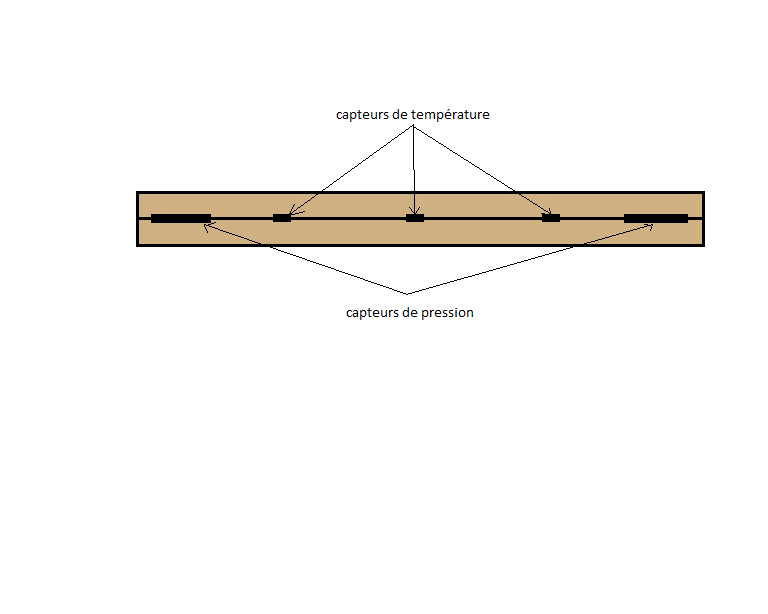
\includegraphics[trim= 9cm 6cm 8cm 2cm,scale=0.8]{cadre_cote1.png}
\caption{\label{fig:cote1} Schéma du cadre de mesure. Coupe vue de coté}
\end{figure}

\begin{figure}[h!]
\centering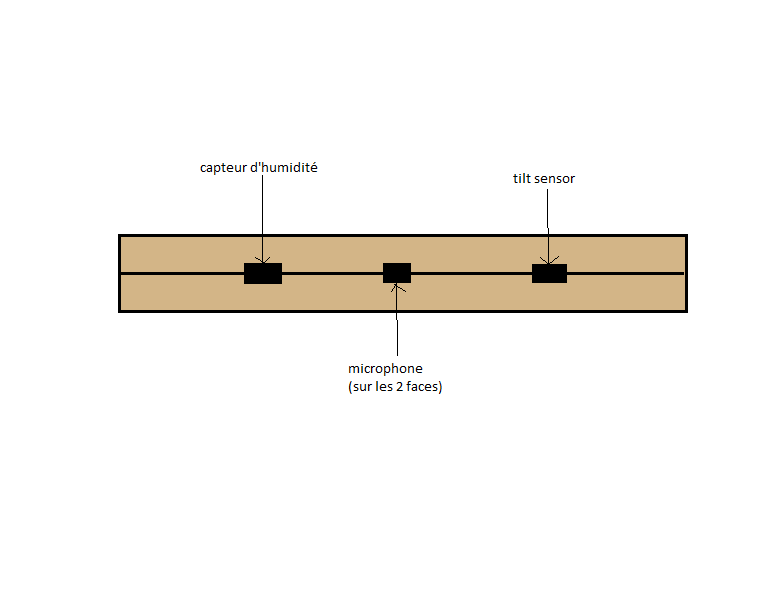
\includegraphics[trim= 5cm 5cm 5cm 5cm,scale=0.8]{cadrecote2.png}
\caption{\label{fig:cote2} Schéma du cadre de mesure. Coupe vue de coté}
\end{figure}

\begin{figure}[h!]
\centering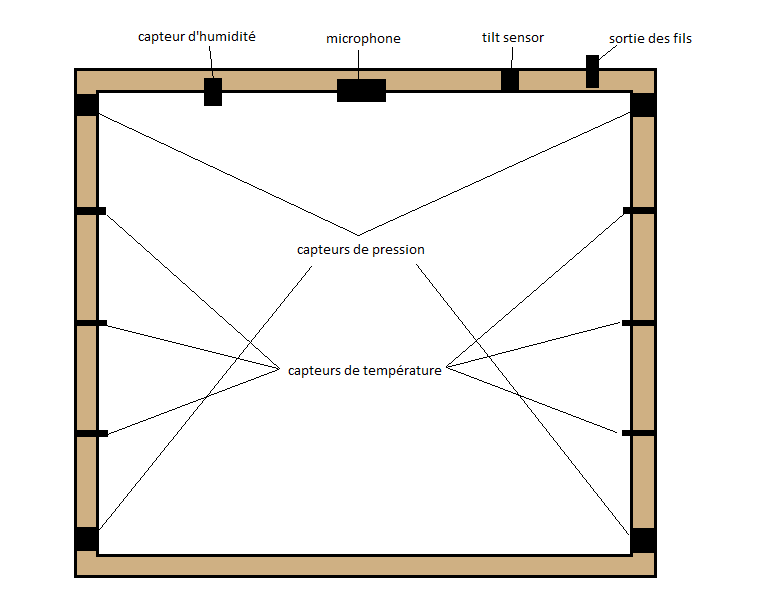
\includegraphics[trim= 1cm 1cm 2cm 3cm,scale=0.8]{cadre_face.png}
\caption{\label{fig:face} Schéma du cadre de mesure. Coupe vue du dessus}
\end{figure}


\clearpage

\section{Architecture physique logicielle}

\vspace{1.5cm}
Dans cette partie nous allons analyser l'architecture logicielle côté logiciel. Elle est divisée en deux parties: Serveur et Arduino. La partie serveur comprend tout qu'est lié au développement du site et les scripts qui contrôlent les logiciels, les backups et l'obtention de données. La partie arduino comprend tous les capteurs et modules, l'énergie et les scripts de contrôle des capteurs et manipulation des données. Ceci est résumé dans le diagramme ci-dessous. 


\begin{figure}[h!]
\centering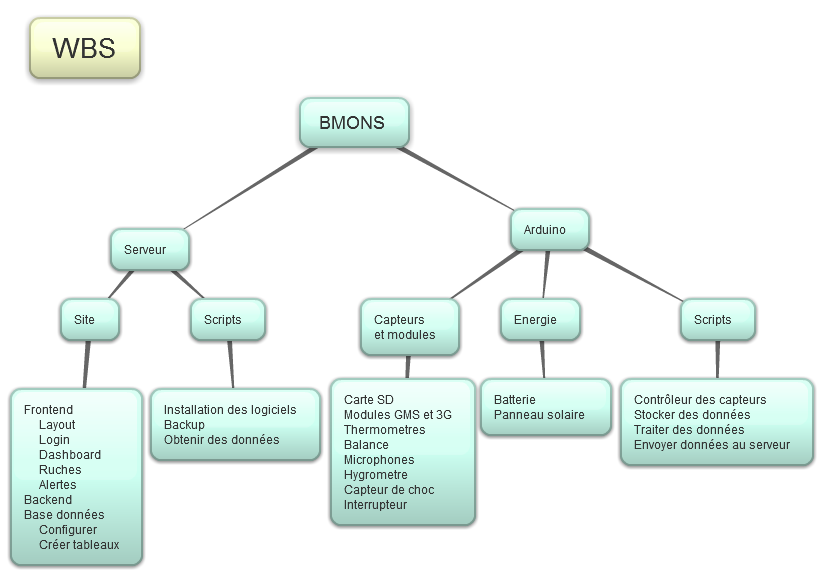
\includegraphics[scale=0.55]{WBS.png}
\caption{\label{fig:SDP} Architecture physique logicielle du système BMONS}
\end{figure}

\clearpage

\subsection{Base de données}

L'organisation de ma base de données se fait comme expliqué sur la figure \ref{fig:UML}.
\begin{figure}[h!]
\centering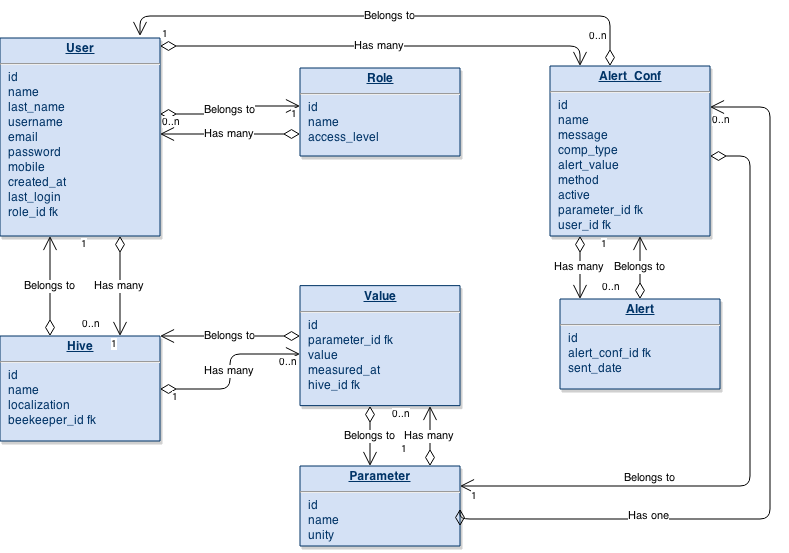
\includegraphics[scale=0.55]{UML.png}
\caption{\label{fig:UML} Modèle de données pour le système BMONS}
\end{figure}

\clearpage

\subsection{Carte Arduino et transmission des données}

Au niveau de la carte Arduino, nous avons commencé à prendre en main les capteurs dès que nous les avions reçus notamment les capteurs de température et de pression. Nous avons commencé à coder un programme qui permettrai de récupérer la température en degrés. Pour la pression, nous récupérons une certaine valeur de résistance. A partir de cela, nous comptons effectuer un étalonnage afin d'en tirer une information sur la masse de la ruche ou des hausses selon la saison et l'envie de l'apiculteur. Cette étalonnage se fera en fonction des informations présentes sur la documentation constructeur du capteur de pression. \\

\begin{figure}[h!]
\centering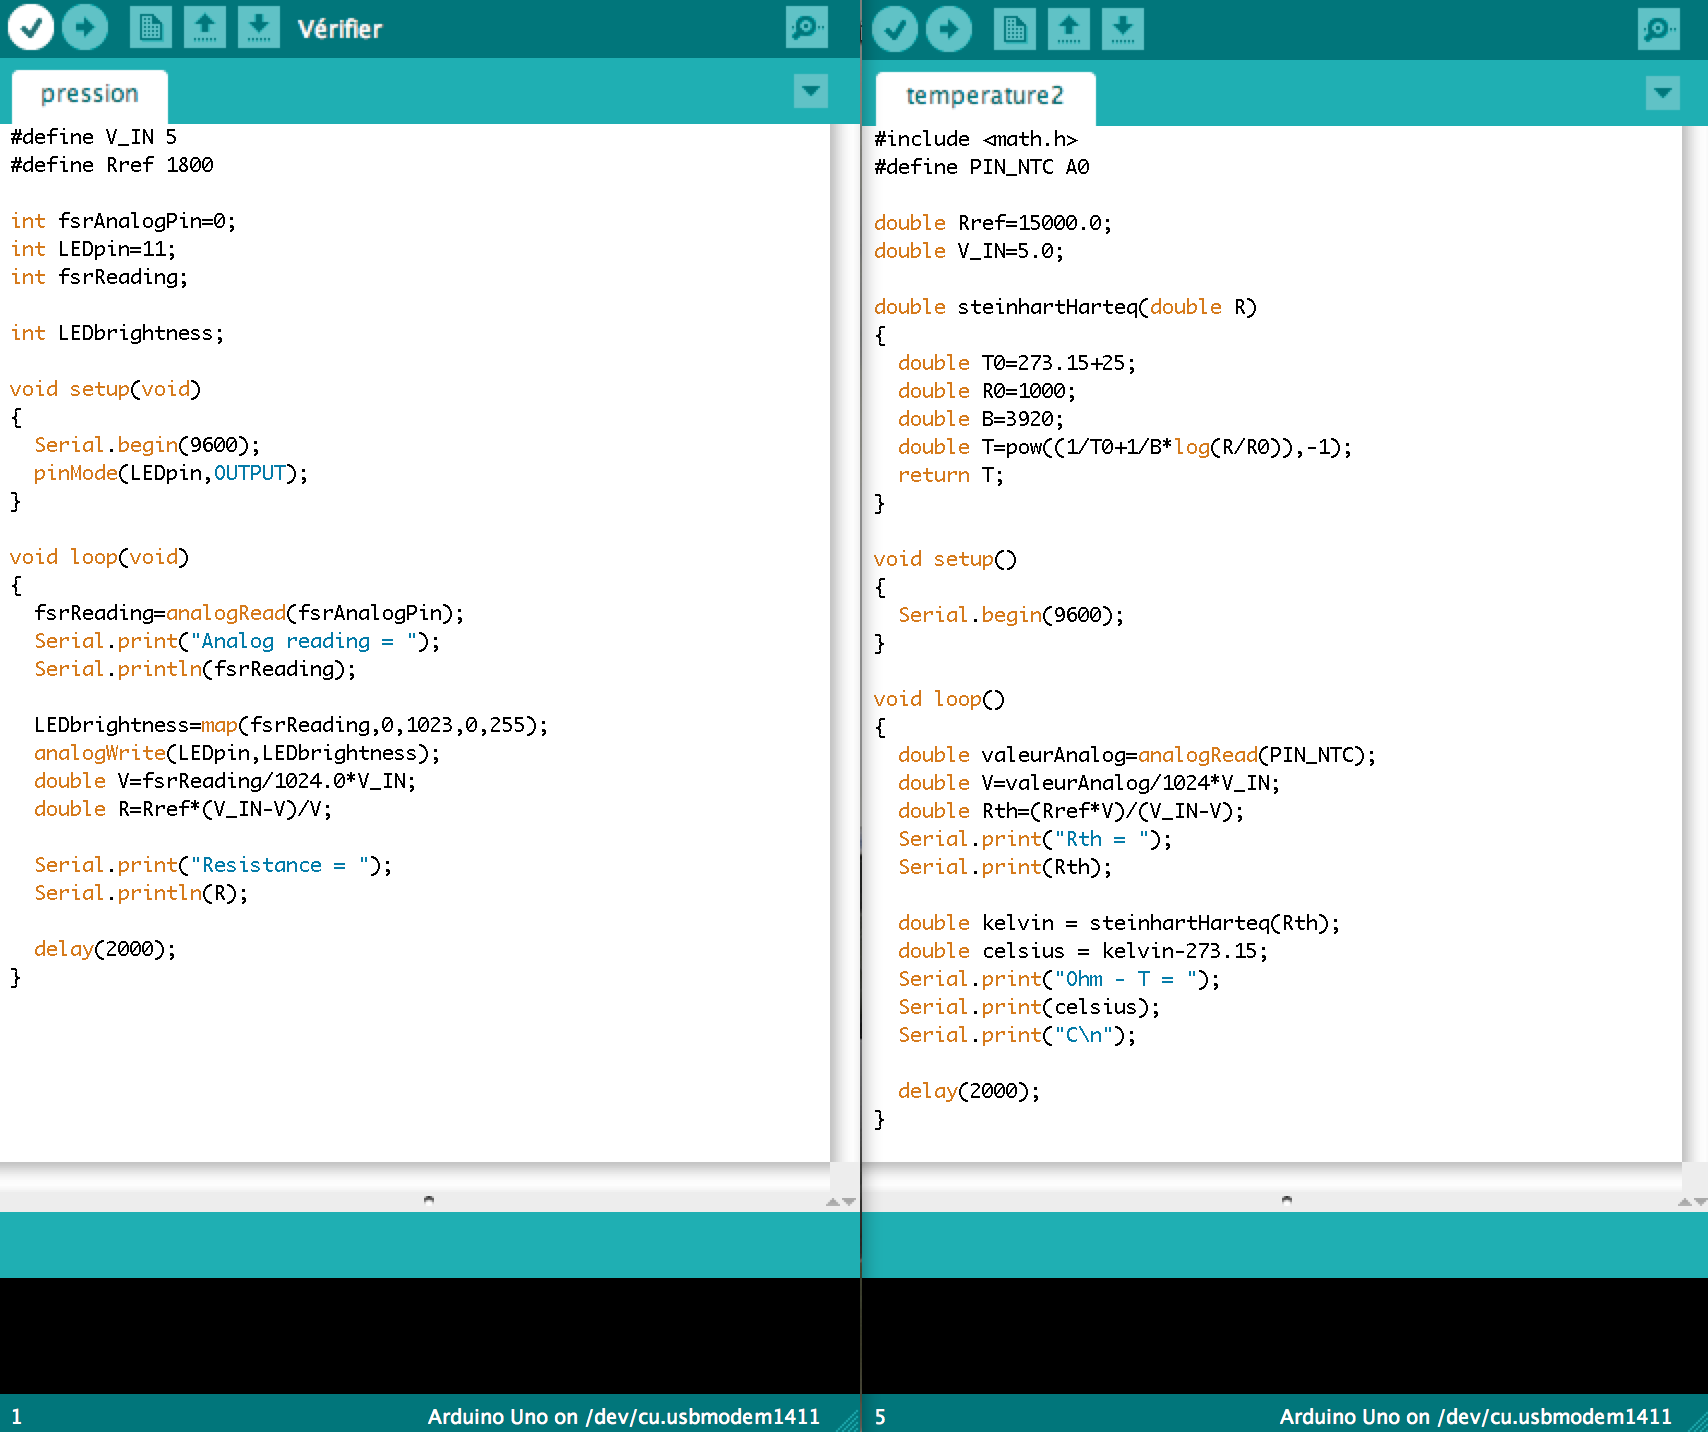
\includegraphics[scale=0.45]{codeArduino.png}
\caption{\label{fig:code} Programmation de la carte Arduino}
\end{figure}  

\clearpage
